\section{Interpretació de l'enunciat i modelat de l'escenari}
En aquest apartat s'expliquen les extensions i suposicions de l'enunciat original,
així el modelat de l'entorn del robot.

Tal i com es demana el programa està parametritzat segons la posició de la càmera,
el punt P que aquesta detecta i l'angle $\alpha$. A més existeixen altres paràmetres
com els punts on es troben les peces originalment i on es deixen al final.

Per altra banda s'ha introduït la possibilitat de fixar un nombre diferent de peces
a cada pila, per tant es poden tenir piles amb diferent número de peces. També
és té amb compte la possibilitat de tenir més d'una peça, o cap, d'algun tipus.

Tots aquests paràmetres es tornen a veure detallats en l'apartat d'explicació del
codi on s'expliquen les \emph{Macros pròpies}\ref{macprop}.

En la figura \ref{escenari} següent es poden veure tots els paràmetres i punts
(marcats amb una estrella) que caracteritzen l'escenari.

\begin{figure}[H]
\begin{center}\label{fig:escenari}
 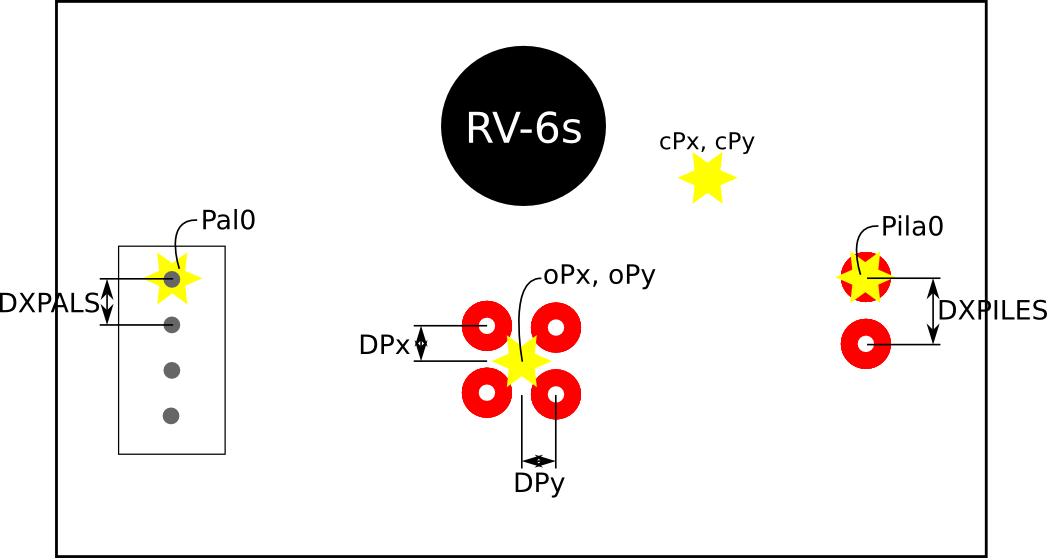
\includegraphics[width=0.8\textwidth]{escenari.png}
 % ordreRotacions.png: 1286x768 pixel, 150dpi, 21.77x13.00 cm, bb=0 0 617 369
\end{center}
  \caption{Escenari del robot}
\end{figure}

La figura es veu complementada amb el llistat de punts emprats a la pràctica.

\begin{minted}[frame=lines, fontsize=\small]{text}
DEF POS Paralisi = (337.16,  -14.95, 270.30, -179.98,  -0.36, -177.39)(7 ,0)
DEF POS Pal0     = (315.50, -550.72, 280.00, -173.00, -67.00,  -90.00)(7, 0)
DEF POS Pila0    = (337.18,  486.51, 280.00, -179.98,  -0.36,  -90.00)(7, 0)
DEF POS Pale0    = (  0.00,    0.00, 280.00, -179.98,  -0.36,  -90.00)(7, 0)
DEF POS PalePT   = (  0.00,    0.00, 280.00,  100.41,  85.49,   98.72)(6, 0)
DEF POS PaleOut0 = (337.00, -450.00, 280.00, -172.92, -66.76,  -90.00)(7, 0)
\end{minted}

Com es detalla en l'apartat de \emph{calcul de punts} \ref{calcpts}
s'ha intentat minimitzar el nombre de punts capturats per tal
de calcular els demes en realció a aquests.

A continuació s'explica l'utlitat de cada punt o posició.

\begin{desciption}
 \item [Paralisi] Guarda la posició del robot en repòs.
 \item [Pal0] Posició del primer pal (amb la pinça tombada).
 \item [Pila0] Posició de la primera pila (amb pinça perpendicular)
 \item [Pale0] Orientació del braç robot per posar peces del palé (amb la pinça
perpendicular).
 \item [PaleOut0] Orientació del braç robot per agafar les peces del palé
(amb la pinça tombada) 
\end{desciption}




\begin{description}
 \item [oPx, oPy] Posició del punt P, en funció de la càmera.
 \item [Pila0] Posició de la primera pila.
 \item [Pal0] Posició del primer pal.
 \item [cPx, cPy] Posició de la càmera que dona el punt P.
 \item [DXPALS] Distància en X entre els pals.
 \item [DXPILES] Distància en X entre les piles.
 \item [DPx] Distància entre el punt P i cada peça en X, és de 5.5cm segons
l'enunciat.
 \item [DPy] Distància entre el punt P i cada peça en Y, és de 5.5cm segons
l'enunciat.
\end{description}

Per simplicitat en la figura no s'han posat els paràmetres Diy ni DLy
ja que en l'escenari original són 0.

Finalment l'enunciat deixa oberta la possibilitat de que fer amb les peces de
tipus 4, en aquest punt s'ha optat per posar-les al pal 4 per aprofitar el codi ja escrit i
així seguir la coherència i estructura dels tipus de peça anteriors. El fet de
no optar per apilar-les en qualsevol punt de l'entorn es perquè en la paletització
ja s'ha demostrat coneixement de com apilar peces i tractar el tipus 4 de manera
diferent als anteriors minvava elegància al codi i l'execució.

\subsection{Moviment del robot}
En primer lloc el robot agafa les peces del les piles inicials.
Aquestes són co\lgem ocades a la zona de paletització. Un cop acabat amb la pinça
tombada agafa les peces començant per les que es troben més a l'esquerra
del braç robot, per co\lgem ocarles als pals. Així doncs al diagrama\ref{fig:recpec}
veim quin seria l'ordre de recollida depenent dels diferents angles.

\begin{figure}[H]
\begin{center}\label{fig:recpec}
 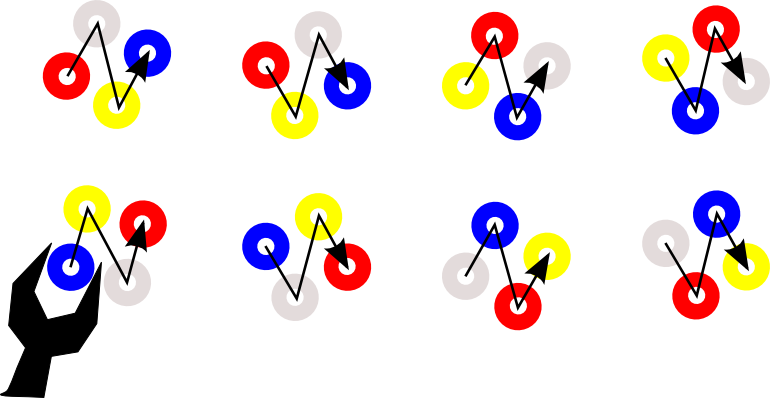
\includegraphics[width=0.8\textwidth]{ordreRotacions.png}
 % ordreRotacions.png: 1286x768 pixel, 150dpi, 21.77x13.00 cm, bb=0 0 617 369
\end{center}
  \caption{Ordre de recollida de les peces segons l'angle $\alpha$}
\end{figure}

Així doncs l'ordre de despaletització depen de l'angle i no del tipus de peça.
Com és pot veure a la figura existeixen 8 possibles casos que es veuen
reflectits en l'explicació del codi font corresponent, secció \ref{casosrot}.

TODO dir mesures de seguretat en el moviment del braç